\documentclass{article}
\usepackage[left=0.75in,top=0.6in,right=0.75in,bottom=0.6in]{geometry} %
\usepackage{graphicx}
\begin{document}
	\begin{center}
		%Name,Address,Contact information (Contact,e-mail), Photograph
		\vspace{10px}
	\textbf{\Huge AYUSH LASOD}
	\vspace{10px}
   \line(3,0){500} \\

~\textbullet~ \textbf{\normalsize PES Institute of Technology, Bengaluru-85} ~\textbullet~ {\textbf{\normalsize ayushlasod@gmail.com}} ~\textbullet~ \textbf{\normalsize 9462243355 }
    \vspace{5px}
    
    
\begin{figure}[h]
	\hspace{200pt}
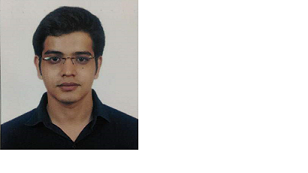
\includegraphics{pic.jpg}
\end{figure}

	%OBJECTIVE

\textbf{\LARGE OBJECTIVE}\\\vspace{10px}
{\large To become associated with a company where I can utilize my skills and gain experience while enhancing the company's productivity
	and reputation.}\\\vspace{15px}

	%EDUCATION

\textbf{\LARGE EDUCATION}\vspace{10px}
\begin{tabular}{|c|c|c|c|c|}\hline
	DEGREE & COLLEGE/SCHOOL & UNIVERSITY & PASSING YEAR & PERCENTAGE \\ \hline
	10th & St. Anselm’s Sr. Sec. School, Bhilwara & CBSE & 2011 & 87.4 \\ \hline
	12th & As' Steward Morris Sr. Sec. School, Bhilwara & CBSE & 2013 & 83.4 \\ \hline
	B.E. (Mech) & PES Institute of Technology, Bengaluru-85 & VTU & 2017 & 74.2 \\ \hline
\end{tabular}\vspace{15px}

	%PROJECTS

\textbf{\LARGE PROJECTS}
\begin{enumerate}
	
	{\large \item •	Final Year Project : Design and Fabrication of Glass Wall Cleaning Robot.\\
		-Presented this Robot Model at e-Yantra Ideas Competition.}
\end{enumerate}\vspace{15px}

\end{center}
\end{document}